% ============================================================================================
% ABEONA Crew Capsule propulsion CAD model -- section for the main report.
% HOW TO USE: paste everything below this comment block into your main .tex file, somewhere
% between \begin{document} and \end{document}, where this section belongs.
% Needs only \usepackage{graphicx} in the main file's preamble (almost every template has it).
% Images: upload these five files to the project (same folder as the main .tex, or a figs/ folder):
%   cad_iso.png  cad_front.png  cad_cut_front.png  cad_cut_iso.png  cad_cut_engine.png
% If your image files have other names, change only the names inside \includegraphics{...}.
% ============================================================================================

\section{Crew Capsule Propulsion CAD Model and Performance Verification}\label{cad:top}

\subsection{Introduction}
This report documents the Onshape CAD model of the Project ABEONA Crew Capsule service-module propulsion system and an
independent check of the main-engine performance. The model contains the 25~kN NTO/MMH main engine, the two propellant
tanks, four helium pressurant bottles, the propellant feed and helium pressurization lines, and reference shells for the
service module, the capsule and the launch escape system (LES).

The engine geometry and the layout were generated by the main-engine design analysis [C1] and were not changed, except
where noted in Sec.~\ref{cad-sec:changes}. The tank size, envelope and LES shape follow the Preliminary Design Review (PDR)
crew-capsule drawing [C2,C3]. The vehicle numbers come from the Crew Capsule tab of \texttt{Mission\_Breakdown.xlsx} [C4].
The ideal performance was re-computed with RocketCEA [C5], which wraps NASA CEA [C6], and compared with the in-house
equilibrium solver used in [C1] (Sec.~\ref{cad-sec:cea}).

\subsection{Model Construction}
The whole model is one parametric Onshape feature, \emph{ABEONA engine and tanks}. It is written in FeatureScript and
generated by a Python script from the analysis outputs \texttt{engine\_profile.csv} and \texttt{layout.json} [C1]. The model
can therefore be rebuilt from the analysis files at any time. Units are millimetres. The origin is at the service-module
(SM) base on the vehicle axis, with $+Z$ up. Figures~\ref{cad-fig:iso} and \ref{cad-fig:front} show the full model.

\begin{figure}[htbp]\centering\graphicspath{{./}{figs/}{images/}{figures/}{Figures/}}
\begin{minipage}{0.48\textwidth}\centering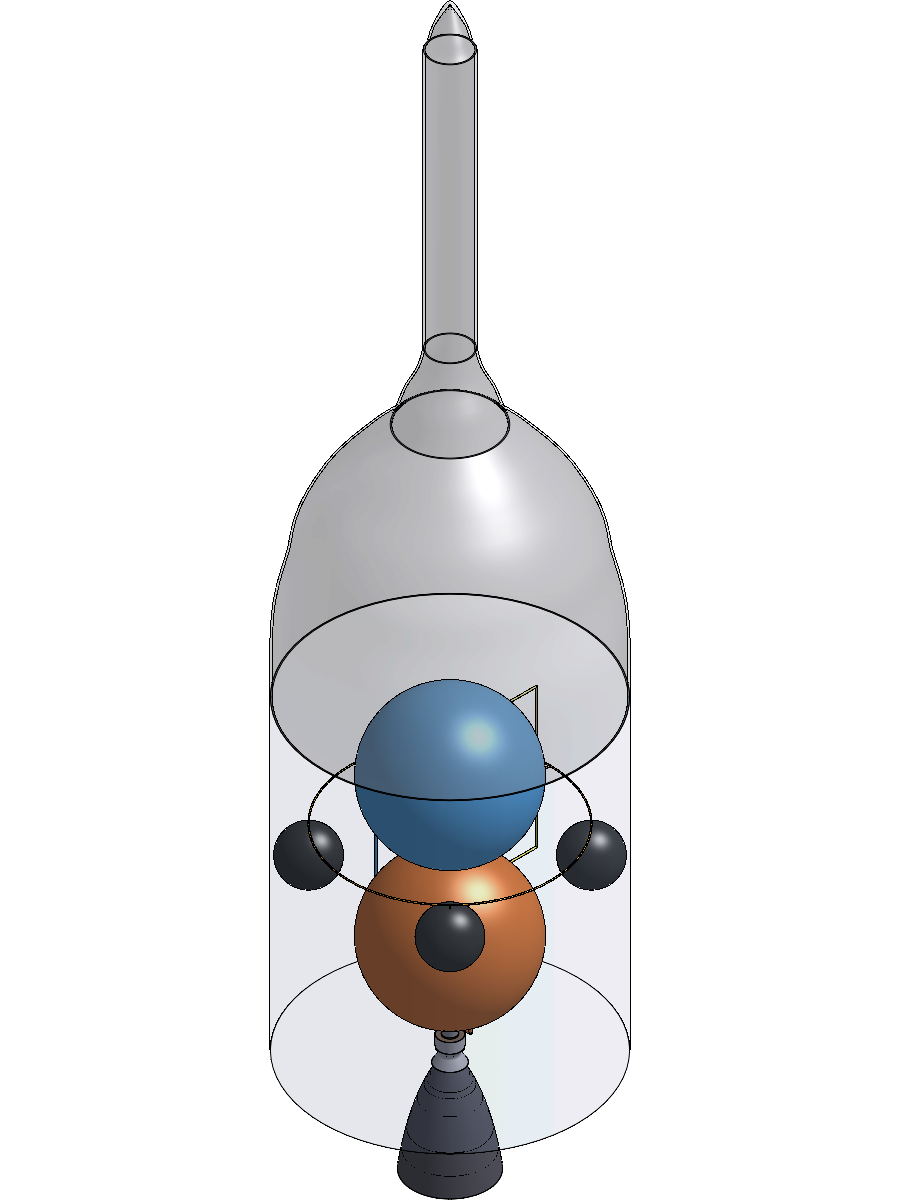
\includegraphics[width=\textwidth]{cad_iso.png}
\caption{Full model, isometric view.}\label{cad-fig:iso}\end{minipage}\hfill
\begin{minipage}{0.48\textwidth}\centering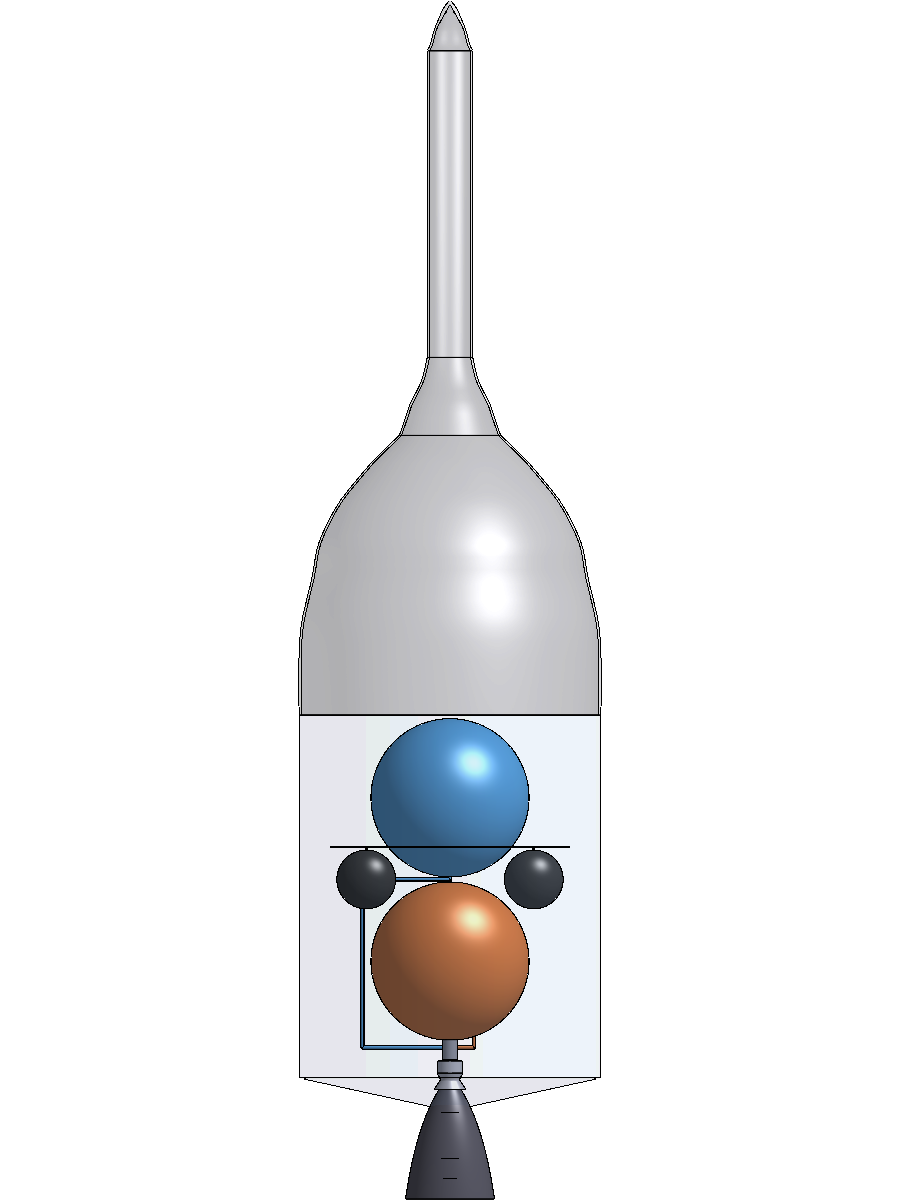
\includegraphics[width=\textwidth]{cad_front.png}
\caption{Full model, front view.}\label{cad-fig:front}\end{minipage}
\end{figure}

\subsubsection{Engine}
The ablative liner, the titanium case and the C-103 nozzle extension are each revolved 360$^\circ$ about the vehicle axis
from the analysis contour. Each is a single smooth body: the gas-side and outer contours are fitted splines through the
contour stations. The cylindrical chamber section is a straight line. The extension is the gas-side spline surface
thickened outward by a constant 0.6~mm. It is trimmed where it meets the liner end face at area ratio 6. The liner, case
and extension stay separate parts because they are different materials.

The injector is a 20~mm 304L plate at chamber diameter with twelve quarter-wave acoustic cavities, each 59.4~mm deep [C1].
The analysis gives only the number and depth of the cavities, so they are modelled as axial \O16~mm bores on a 100~mm
pitch radius. The valve, gimbal and head stack is a cylinder 350~mm long, from the injector face to the gimbal plane. Its
density is set so that the cylinder carries the 44~kg budgeted in [C1] for valves, gimbal actuators and miscellaneous items.

\subsubsection{Tanks, pressurant and envelope}
The NTO and MMH tanks are Ti-6Al-4V spherical shells. The helium bottles are spherical shells with a 20~mm wall and a
density chosen to carry the composite overwrapped pressure vessel (COPV) mass of [C1]. The SM envelope (4.98~m diameter,
6~m long, 0.5~m aft cone) is a transparent reference body. The capsule and LES outer shape is a 20~mm reference shell with
no mass. It was traced from the PDR drawing [C3], scaled to the 4.98~m SM diameter and the 11.8~m height from the SM top
to the LES tip. The drawing's 0.41~m dimension lands on the LES nose. The tower, as drawn, is about 0.74~m in diameter,
and the model follows the drawing.

\subsubsection{Cut view}
The feature has a \emph{Cut view} checkbox that removes the $-Y$ half of every body. This exposes the engine section, the
hollow tanks and bottles, and the feed lines, which lie in the cut plane (Figs.~\ref{cad-fig:cutfront}--\ref{cad-fig:cutengine}).
Mass properties must be read with the cut view off. Onshape's own section-view tool gives the same picture without
changing the model.

\begin{figure}[htbp]\centering\graphicspath{{./}{figs/}{images/}{figures/}{Figures/}}
\begin{minipage}{0.48\textwidth}\centering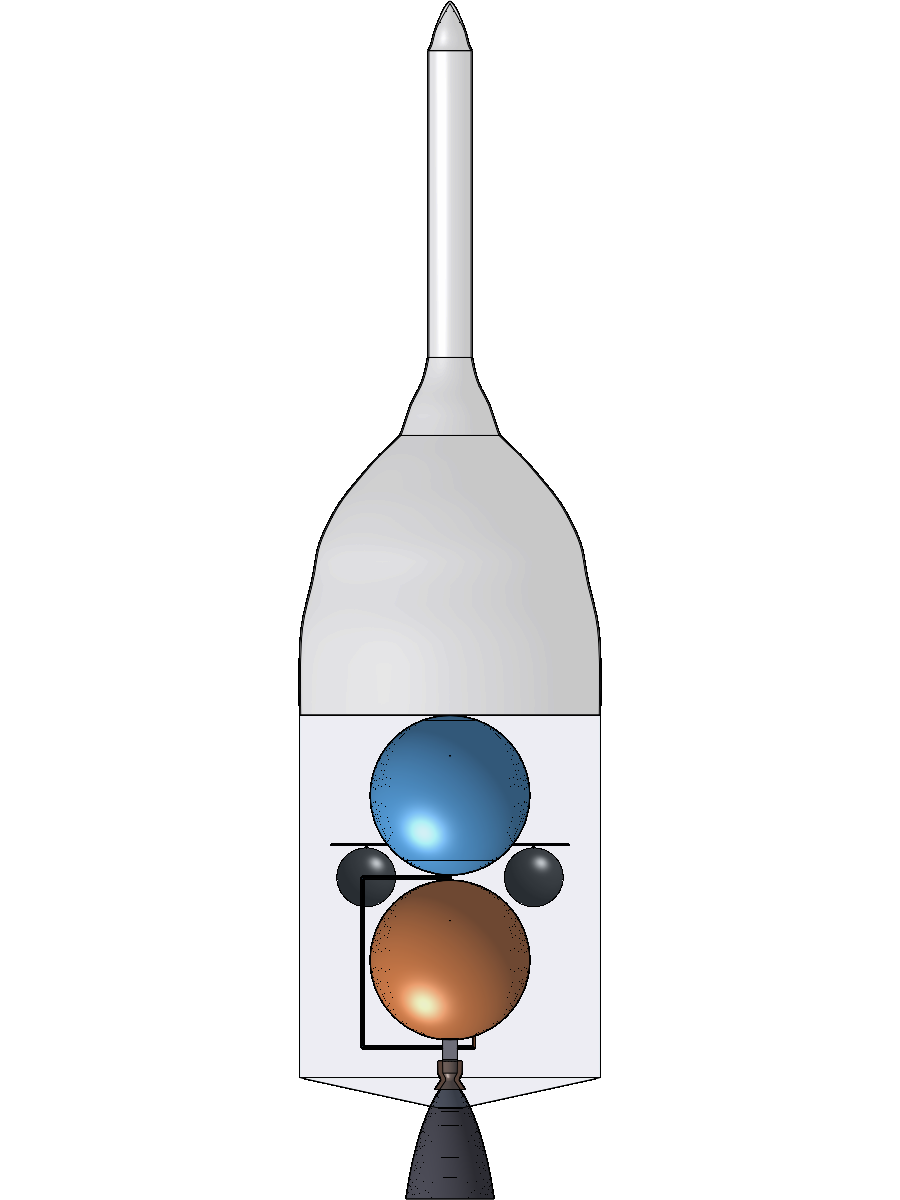
\includegraphics[width=\textwidth]{cad_cut_front.png}
\caption{Cut view, front.}\label{cad-fig:cutfront}\end{minipage}\hfill
\begin{minipage}{0.48\textwidth}\centering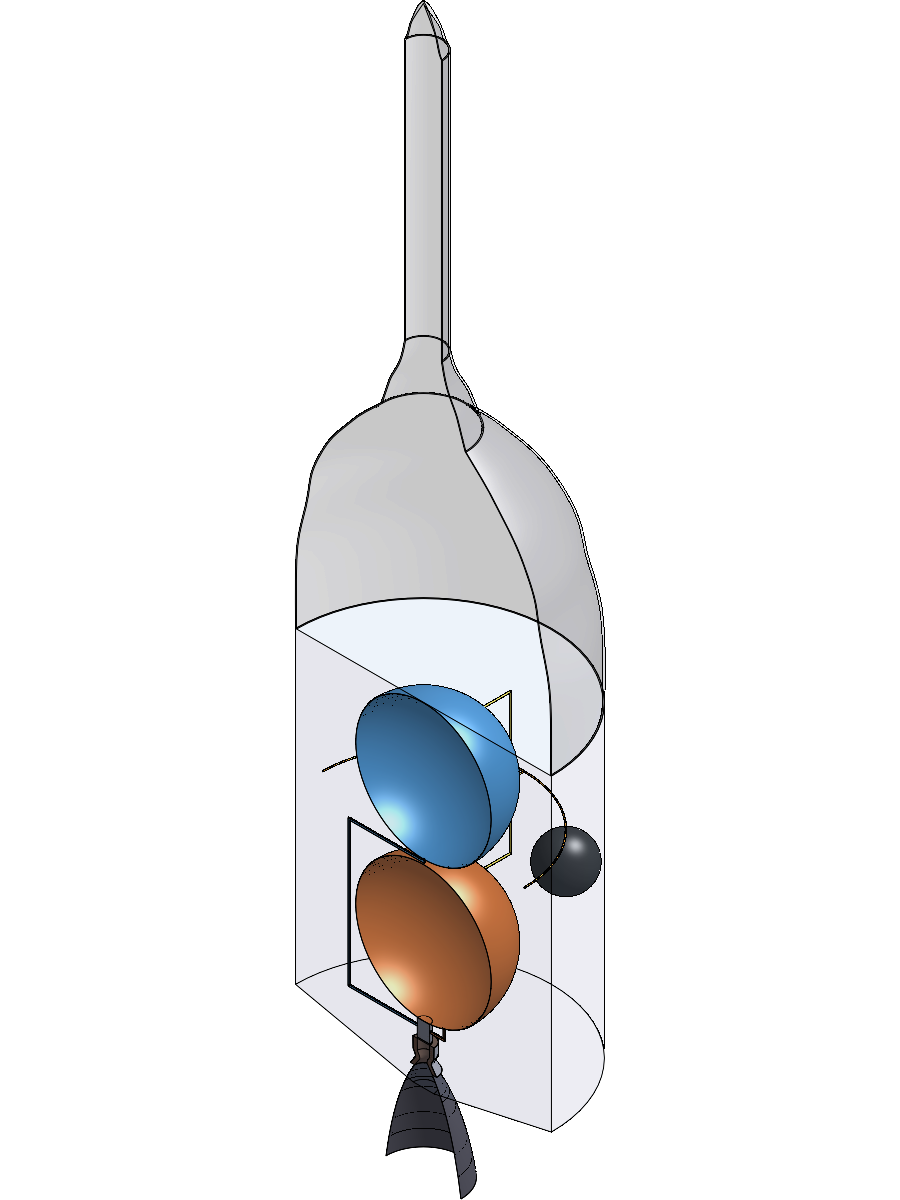
\includegraphics[width=\textwidth]{cad_cut_iso.png}
\caption{Cut view, isometric.}\label{cad-fig:cutiso}\end{minipage}
\end{figure}
\begin{figure}[htbp]\centering\graphicspath{{./}{figs/}{images/}{figures/}{Figures/}}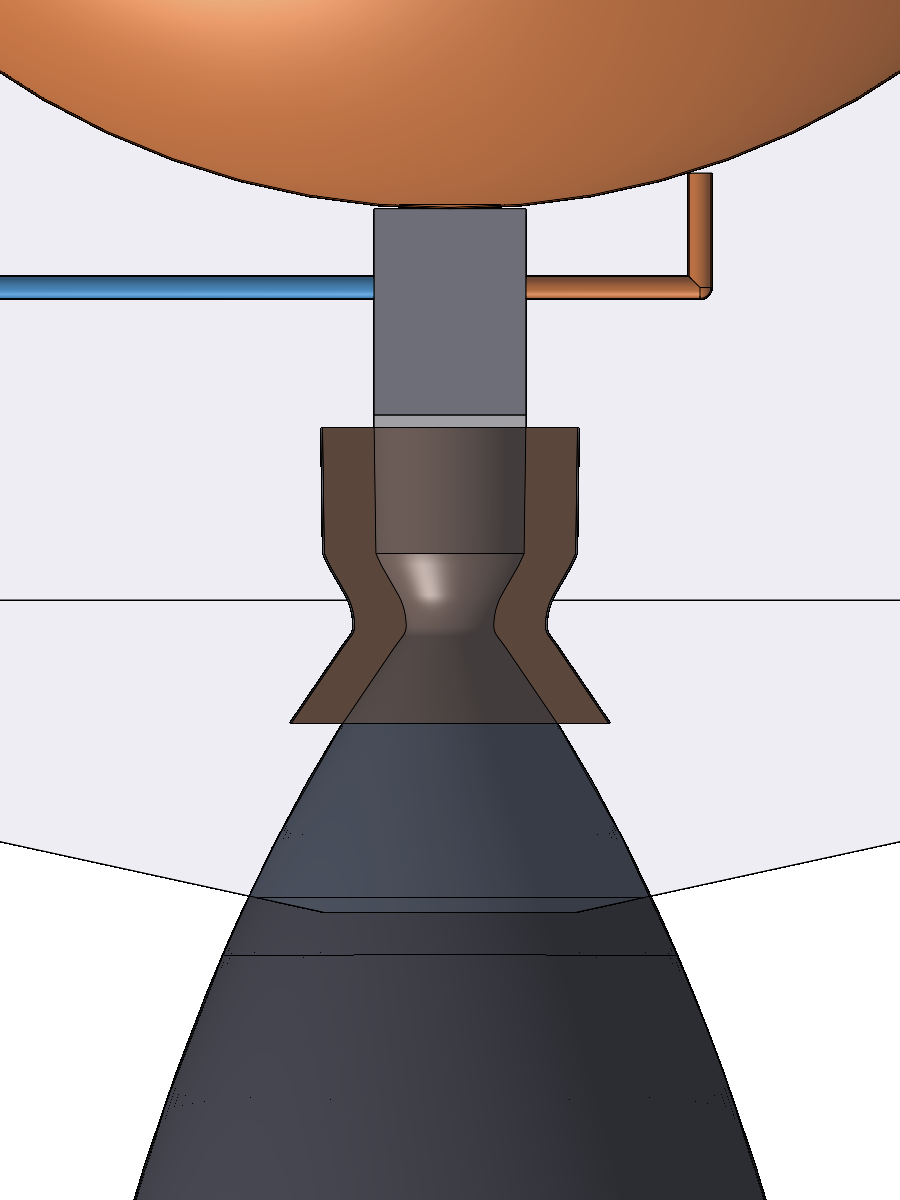
\includegraphics[width=0.6\textwidth]{cad_cut_engine.png}
\caption{Cut view of the engine: head stack, injector, silica-phenolic liner and Ti case, throat, and the start of the
C-103 extension, with the NTO (right) and MMH (left) feed lines entering the valve stack.}\label{cad-fig:cutengine}\end{figure}

\subsection{Changes from the Analysis Layout}\label{cad-sec:changes}
\begin{itemize}
\item \textbf{Tank size.} The tanks follow the PDR drawing [C3]: 2.6~m inner diameter, 9.203~m$^3$ each. The wall is
scaled from [C1] to 2.14~mm, which keeps the same maximum operating pressure and allowable stress. The two tanks are the
same size by design. At O/F~1.65, the NTO (1,440~kg/m$^3$) and MMH (875~kg/m$^3$) loads occupy 9.08 and 9.06~m$^3$
(PDR requirements 1.2.2-01/02 [C2]). The analysis in [C1] enlarged the tanks to 2.63~m for 5~\% ullage. With 2.6~m tanks,
the free volume is only 1.3~\% (NTO) and 1.6~\% (MMH), which is below the usual 3--5~\%. This is an open item: either
return to 2.63~m or offload about 3~\% of the propellant.
\item \textbf{Tank stacking.} The analysis placed the NTO tank from its inner diameter, so its 2.16~mm wall overlapped
the head stack by 19.4~cm$^3$. Both tanks now sit on their outer surfaces. The NTO centre is at $z = 1{,}928$~mm and
the MMH centre at $z = 4{,}632$~mm, with a 100~mm gap between the tanks and 65~mm clearance to the SM top. The helium
bottles keep the same rules as before: 50~mm above the NTO tank and 50~mm from the SM wall.
\item \textbf{Lines added.} The analysis sized the feed lines but did not lay them out. The routing and the helium line
sizes are new (Sec.~\ref{cad-sec:lines}).
\end{itemize}
A two-bottle helium layout ($2\times1.206$~m COPVs, same total volume) was also checked. It fitted with 376~mm tank
clearance, but the four-bottle baseline was retained.

\subsection{Feed and Pressurization Lines}\label{cad-sec:lines}
The system is pressure-fed with regulated helium. Four 31~MPa COPVs supply a regulator that holds both tank ullages at
1.33~MPa, and the tank pressure drives the propellants to the engine [C1]. All lines are 321 stainless steel
(Table~\ref{cad-tab:lines}). The propellant line size is taken from the feed analysis in [C1]. The helium lines were sized
for this model:
\begin{itemize}
\item \textbf{High-pressure line.} The governing load is the 31~MPa bottle pressure. A 3/8~in~$\times$~0.065~in tube
then sees a 90~MPa hoop stress, a factor of 5.7 on ultimate.
\item \textbf{Low-pressure lines.} These are sized by the helium flow that replaces the outflowing propellant, 3.4~L/s
per tank. A 3/4~in~$\times$~0.049~in tube keeps the helium velocity near 16~m/s.
\end{itemize}

The regulator and check-valve panel is a lumped 10~kg block. Valves, filters, the flexible sections each feed line needs
where it crosses the gimbal, the propellant management devices and the line supports are not modelled.

\begin{table}[htbp]\centering\small\caption{Feed and pressurization lines.}\label{cad-tab:lines}
{\footnotesize\setbox0=\hbox{\begin{tabular}{p{0.13\linewidth}p{0.17\linewidth}p{0.24\linewidth}p{0.31\linewidth}}\hline
Line & OD $\times$ wall & Basis & Route \\\hline
NTO feed & 1.5~in $\times$ 0.065~in & 4.95~kg/s at 3.6~m/s; 64~kPa line loss [C1] & NTO lower dome ($r = 400$~mm), down, into the $+X$ side of the valve stack at $z = 500$~mm \\
MMH feed & 1.5~in $\times$ 0.065~in & 3.00~kg/s at 3.6~m/s; 50~kPa line loss [C1] & MMH bottom pole, through the tank gap, down at $x = -1{,}450$~mm outside the NTO tank, into the $-X$ side of the valve stack \\
He high pressure & 0.375~in $\times$ 0.065~in & 31~MPa; hoop stress 90~MPa (factor 5.7 on ultimate) & COPV top outlets to a ring manifold ($r = 1{,}961$~mm, $z = 3{,}819$~mm), then to the regulator \\
He low pressure & 0.75~in $\times$ 0.049~in & 1.33~MPa; about 16~m/s at 3.4~L/s per tank & Regulator ($+Y$, $r = 1{,}700$~mm) to each tank's upper dome, 60$^\circ$ from the top pole \\
\hline\end{tabular}}\ifdim\wd0>\linewidth\resizebox{\linewidth}{!}{\box0}\else\box0\fi}\end{table}

\subsection{Nozzle Extension Wall}
The C-103 extension wall is 0.6~mm thick. Internal pressure does not size it. The gas pressure is 19.9~kPa at the
attach station (area ratio 6, Mach 3.0) and 0.44~kPa at the exit. With $\sigma = p r / t$, the hoop stress is 5.7~MPa
at the attach station and 0.5~MPa at the exit, which is far below the strength of C-103 at its 1,389~K peak temperature
(1,600~K limit) [C1].

Thickness also does not affect the wall temperature. A radiation-cooled skirt runs at radiation equilibrium, so a thicker
wall only adds mass. The real sizing loads are stiffness against vibration, gimbal and handling loads, and the attach
flange. The mass budget covers these with a 25~\% allowance for stiffening rings, the flange and the coating (40.7~kg
against 32.5~kg for the bare wall) [C1]. The CAD shows the bare wall. A taper from about 1.0~mm at the flange to 0.6~mm at
the exit, with two or three hat-section stiffening rings, would represent the hardware more fully without changing the
thermal design.

\subsection{Mass Properties}
Onshape nominal mass properties, with the cut view off, are compared with the analysis mass build-up [C1] in
Table~\ref{cad-tab:cadmass}. The densities used are silica phenolic 1,750, Ti-6Al-4V 4,430, C-103 8,860, 304L 7,900 and
321 stainless 8,030~kg/m$^3$. Items marked ``lumped'' have a density chosen to match the budget. The modelled masses are
bare geometry. The analysis values also include flanges, rings, manifolds and tank fittings that are not drawn.

\begin{table}[htbp]\centering\small\caption{CAD mass properties against the analysis mass build-up.}\label{cad-tab:cadmass}
{\footnotesize\setbox0=\hbox{\begin{tabular}{p{0.23\linewidth}p{0.13\linewidth}rrp{0.25\linewidth}}\hline
Part & Material & CAD, kg & Analysis, kg & Note \\\hline
Ablative liner & silica phenolic & 66.13 & 66.38 & \\
Chamber case & Ti-6Al-4V & 6.47 & 10.03 & analysis adds 3~kg of flanges \\
Nozzle extension & C-103 & 33.23 & 40.65 & analysis: 32.5~kg bare $\times$ 1.25 \\
Injector plate & 304L & 6.94 & 10.00 & analysis includes a 2.6~kg manifold \\
Head, valve and gimbal stack & lumped & 44.00 & 44.00 & valves, actuators, miscellaneous \\
NTO tank (bare shell) & Ti-6Al-4V & 201.28 & 271.92 & 2.6~m ID; analysis value includes more than the shell \\
MMH tank (bare shell) & Ti-6Al-4V & 201.28 & 271.22 & as above \\
Helium COPVs ($\times$4) & lumped & 379.94 & 379.94 & \\
Feed lines (NTO / MMH) & 321 SS & 0.70 / 8.50 & & \\
He lines (high / low pressure) & 321 SS & 4.17 / 2.01 & & \\
Lines total & & 15.38 & 12.93 & the MMH line is 5.6~m long because it routes around the NTO tank \\
Regulator panel & lumped & 10.00 & -- & part of the 40~kg components budget \\
\hline\end{tabular}}\ifdim\wd0>\linewidth\resizebox{\linewidth}{!}{\box0}\else\box0\fi}\end{table}

\subsection{Interference Check}
Every pair of the 17 hardware bodies (136 pairs) was intersected on copies in Onshape. There is no interference. The
largest overlap of any pair is $4\times10^{-5}$~mm$^3$, which is numerical noise at tangent contacts. Connected parts
meet with gaps of 0--0.12~mm. The 0.12~mm gap is at the MMH outlet, where the flat tube end meets the curved dome.
Selected clearances:
\begin{itemize}
\item NTO to MMH tank: 95.7~mm.
\item Bottles to the SM wall: 50~mm.
\item Bottles to the propellant tanks: 601~mm.
\end{itemize}
Against the SM envelope, only the C-103 extension lies outside (3.27~L). This is expected, because the nozzle exit is
2.01~m below the SM base and the aft cone is only 0.5~m deep.

\subsection{Performance Verification with RocketCEA}\label{cad-sec:cea}
The ideal design point of [C1] was re-run with RocketCEA 1.2.3 [C5]: N$_2$O$_4$/MMH, $P_c = 0.862$~MPa, O/F~1.65, area
ratio 108, infinite-area combustor, with frozen flow frozen at the chamber.

RocketCEA's built-in propellant cards use different heats of formation from the NASA database used in [C1]. For example,
N$_2$O$_4$(l) is $-19.56$~kJ/mol in RocketCEA against $-17.55$~kJ/mol in the database. The comparison therefore uses
custom cards with the database values and the 293.15~K propellant temperature of [C1]. The default cards are shown for
reference (Table~\ref{cad-tab:cea}).

\begin{table}[htbp]\centering\small\caption{Ideal vacuum performance: analysis solver [C1] against RocketCEA.}\label{cad-tab:cea}
{\footnotesize\setbox0=\hbox{\begin{tabular}{lrrrrr}\hline
 & Analysis & RocketCEA, & & RocketCEA, & \\
Quantity & [C1] & same basis & Diff. & default cards & Diff. \\\hline
$T_c$, K & 3{,}042.3 & 3{,}045.7 & +0.11~\% & 3{,}044.6 & +0.08~\% \\
$\mathcal{M}_c$, g/mol & 20.42 & 20.41 & $-$0.03~\% & 20.41 & $-$0.02~\% \\
$c^*$, shifting, m/s & 1{,}737.9 & 1{,}739.4 & +0.08~\% & 1{,}738.9 & +0.06~\% \\
$C_{F,vac}$, shifting & 1.9276 & 1.9281 & +0.03~\% & 1.9280 & +0.02~\% \\
$I_{sp,vac}$, shifting, s & 341.50 & 341.99 & +0.14~\% & 341.87 & +0.11~\% \\
Exit pressure, shifting, Pa & 429.9 & 430.3 & +0.09~\% & 430.2 & +0.06~\% \\
$c^*$, frozen, m/s & 1{,}698.6 & 1{,}699.8 & +0.07~\% & 1{,}699.4 & +0.05~\% \\
$C_{F,vac}$, frozen & 1.8753 & 1.8753 & 0.00~\% & 1.8753 & 0.00~\% \\
$I_{sp,vac}$, frozen, s & 324.71 & 325.04 & +0.10~\% & 324.97 & +0.08~\% \\
\hline\end{tabular}}\ifdim\wd0>\linewidth\resizebox{\linewidth}{!}{\box0}\else\box0\fi}\end{table}

Every quantity agrees within 0.3~\%, exit temperature included. This confirms the ideal performance on which the
delivered 320.8~s specific impulse in [C1] is built.

\subsection{Compliance with the Mission Breakdown}\label{cad-sec:mb}
The design was checked against every value in the Crew Capsule tab of the mission breakdown spreadsheet [C4]
(Table~\ref{cad-tab:mb}). All values are met except the propellant volume at high propellant temperature. NTO expands
as it warms. In the 2.6~m PDR tanks (9.203~m$^3$), the 13,076~kg NTO load leaves 2.9~\% free volume at 10~$^\circ$C,
1.35~\% at 20~$^\circ$C and 0.56~\% at 25~$^\circ$C, and it does not fit at the 32~$^\circ$C hot case ($-0.57$~\%).
The MMH tank keeps 0.8~\% at 32~$^\circ$C. The analysis tank sizes (2.633~m MMH, 2.635~m NTO) give 3.4~\% at 32~$^\circ$C
and fit the SM if the gap between the tanks is reduced from 100 to 90~mm.

\begin{table}[htbp]\centering\small\caption{Design against the Crew Capsule mission breakdown.}\label{cad-tab:mb}
{\footnotesize\setbox0=\hbox{\begin{tabular}{p{0.19\linewidth}p{0.27\linewidth}p{0.38\linewidth}}\hline
Item & Mission breakdown & Design \\\hline
Thrust, engines & 25~kN, 1 engine & 25~kN vacuum, 1 engine (met) \\
Specific impulse & 280~s & 320.8~s delivered, 303.5~s pessimistic (met) \\
$\Delta v$ & 2,209~m/s & 2,531~m/s, 2,394~m/s pessimistic (met) \\
$M_0$, $M_p$, $M_b$ & 38,000 / 21,000 / 17,000~kg & unchanged (met) \\
$\dot m \times t_b$ & 9.10~kg/s $\times$ 2,307~s & 7.94~kg/s $\times$ 2,644~s = 21,000~kg; liner life 3,305~s (met) \\
$T/W$ at the Moon & 0.405 full, 0.905 empty & unchanged (met) \\
Structural mass $M_s$ & 6,500~kg & propulsion system 1,373~kg, 21.1~\% (met) \\
Propellant volume & 21,000~kg at O/F 1.65 & fits up to about 28~$^\circ$C in 2.6~m tanks (open item) \\
\hline\end{tabular}}\ifdim\wd0>\linewidth\resizebox{\linewidth}{!}{\box0}\else\box0\fi}\end{table}

\subsection{Conclusions}
The service-module propulsion system is modelled as one parametric Onshape feature built directly from the analysis
outputs. It includes the engine, the PDR-size tanks, four helium bottles, sized feed and pressurization lines, and
reference shells for the SM, the capsule and the LES. The model has no interferences, and its masses agree with the
analysis budget once the undrawn flanges, rings and fittings are accounted for. The 0.6~mm C-103 extension wall is
adequate for pressure and temperature; its sizing loads are stiffness and handling, which are covered by the ring
allowance. RocketCEA reproduces the analysis performance within 0.3~\%. Two items remain open: the 1.3--1.6~\% ullage of
the 2.6~m PDR tanks, and the flex sections the feed lines need across the gimbal.

\subsection*{References for this section}
{\small\begin{description}
\item[{[C1]}] [Your Name], ``Project ABEONA Crew Capsule Main Engine: Thrust Chamber, Feed System, and Pressurization Design,'' design report, October 2026.
\item[{[C2]}] Kempf, A., Bratt, E., LeRoy, M., Bernal, R., Wiser, S., and Rouland, S., ``Project ABEONA Preliminary Design Report,'' unpublished class report, 2026.
\item[{[C3]}] Kempf, A., Bratt, E., LeRoy, M., Bernal, R., Wiser, S., and Rouland, S., ``Preliminary Design Review, Project ABEONA,'' unpublished class presentation, slide 7 (Crew Capsule), 2026.
\item[{[C4]}] Project ABEONA, \texttt{Mission\_Breakdown.xlsx}, Crew Capsule tab, 2026.
\item[{[C5]}] Taylor, C., ``RocketCEA,'' Python wrapper for NASA CEA, version 1.2.3, rocketcea.readthedocs.io.
\item[{[C6]}] Gordon, S. and McBride, B. J., ``Computer Program for Calculation of Complex Chemical Equilibrium Compositions and Applications,'' NASA RP-1311, 1994.
\end{description}}
